
\documentclass[12pt]{memoir}
\def\nsigla{MATH667}
\def\nsiglahead{Representation Theory Project}
\def\nsemestre{SP}
\def\nyear{26}
\def\nterm{SP}
\def\nprofesor{Rachel Pries}
\def\nextra{Handout}
\def\nlang{ENG}

\input{../../../headerVarillyDiff}

% Fix numbering for memoir class without chapters
\renewcommand{\thesection}{\arabic{section}}
\renewcommand{\thefigure}{\arabic{figure}}

\begin{document}

\section{Objective and Introduction}

\begin{itemize}
    \item \textbf{Objective}\\ 
    Understand the definition of Lie algebra representations, focusing specifically on $\mathfrak{sl}_2$. Explore the properties of these representations through a combinatorial lens.
    
    \item \textbf{Representations of Lie Algebras}\\
    A Lie algebra \(\g\) is a vector space with a Lie bracket 
    \[
    \bonj{-,-}:\g\x\g\to\g,
    \]
    which is bilinear, alternating, and satisfies the Jacobi identity. Given a vector space \(V\), a representation of a Lie algebra is a map
    \[
    \rho\:\g\to\End(V),
    \]
    where the bracket in \(\End(V)\) is the matrix commutator and the map preserves the Lie bracket structure.
    \item \textbf{The Lie Algebra $\mathfrak{sl}_2$}\\
    The Lie algebra $\mathfrak{sl}_2(\mathbb{C})$ is
    \[
    \gsl_2=\set{A\in M_2(\bC):\ \tr(A)=0}
    \]
    It is generated by:
    \[
    E = \begin{pmatrix} 0 & 1 \\ 0 & 0 \end{pmatrix}, \quad F = \begin{pmatrix} 0 & 0 \\ 1 & 0 \end{pmatrix}, \quad H = \begin{pmatrix} 1 & 0 \\ 0 & -1 \end{pmatrix}.
    \]
    With the Lie bracket \([X,Y]=XY-YX\), the generators satisfy the relations:
    \[
    [E, F] = H, \quad [H, E] = 2E, \quad [H, F] = -2F.
    \]

    \item So we may outline how we're going to complete our objective:
    \begin{enumerate}
        \item Understand the irreducible representations of $\mathfrak{sl}_2$ and view examples. 
        \item Visualize the representations as graphs and connect them with crystal base theory.
        \item Analyze tensor products of representations, derive the Clebsch-Gordan rule.
        \item Connect the representation theory of \(\gsl_2\) to crystals of \(\set{1,2}\)-words.
    \end{enumerate}
\end{itemize}
\vfill
\newpage
\section{Classifying Irreducible Representations}

\begin{Th}
    If \(V\) is an irreducible representation of \(\gsl_2\), it decomposes into weight spaces as:
    \[
    V = \bigoplus_{\al \in \Spec H} V_\al,
    \]
    where \(V_\al\) are the 1-dimensional eigenspaces of \(H\). 
\end{Th}

Each irreducible representation can be visualized as a graph whose vertices correspond to the eigenspaces of \(H\) and the directed edges to the actions of the generators.

\begin{Ex}
The \emph{trivial representation} is \(\bC\) where \(E, F\), and \(H\) map to ``multiplication by 0''. The only eigenvalue of \(H\) is 0, so the decomposition is trivially \(V = V_0\).
\end{Ex}

\begin{figure}[h]
    \centering
    \begin{minipage}{0.45\textwidth}
        \centering
        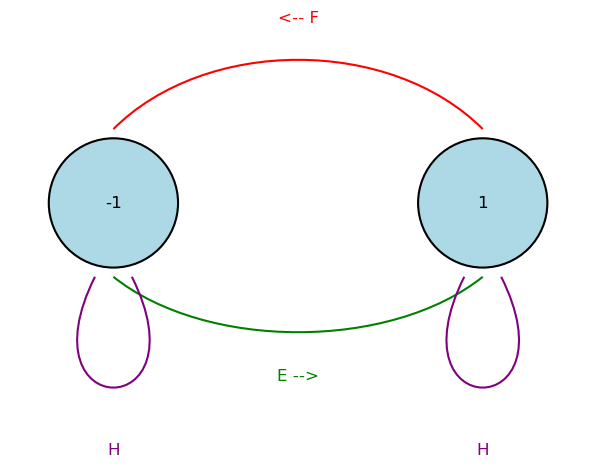
\includegraphics[width=0.65\textwidth]{figs/V1graph.png}
        \caption{Graph of the standard representation $V^{(1)}$}
    \end{minipage}
    \hfill
    \begin{minipage}{0.45\textwidth}
        \centering
        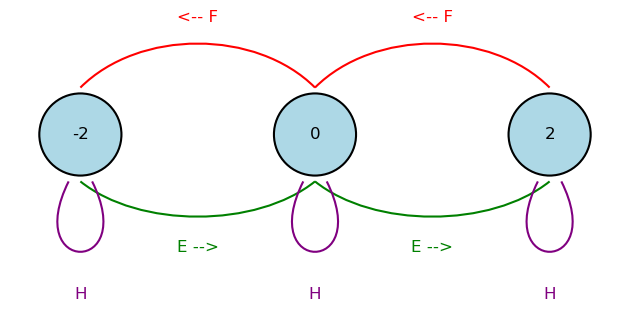
\includegraphics[width=\textwidth]{figs/V2graph.png}
        \caption{Graph of the adjoint representation $V^{(2)}$}
    \end{minipage}
\end{figure}

\begin{Ex}
For the \emph{standard representation}, the map is 
\[
\rho: \gsl_2 \to \End(\bC^2)
\] 
which happens to be the inclusion, i.e. the matrices map to themselves. In this case,
\[
He_1=e_1\word{and}He_2=-e_2,
\]
resulting in the decomposition \(V^{(1)} = \bC^2 = \gen(e_1) \oplus \gen(e_2) = V_{1} \oplus V_{-1}\).
\end{Ex}

\begin{Ex}
The \emph{adjoint representation} is determined by the adjoint map 
\[
\Ad: \gsl_2 \to \End(\gsl_2),\quad \Ad_X(Y) = [X, Y].
\]
Observe that via the commutation relations 
\[
    [E, F] = H, \quad [H, E] = 2E, \quad [H, F] = -2F,
\]
we have that \(V^{(2)}=V_2\oplus V_0\oplus V_{-2}\).
\end{Ex}

\section{Tensor Products}

We may tensor representations to obtain new representations. The Clebsch-Gordan rule gives us a way to decompose the tensor product $V^{(n)} \otimes V^{(m)}$ into irreducibles.

\begin{Th}
    If $n \geq m$, we have:
$$ V^{(n)} \otimes V^{(m)} \cong V^{(n+m)} \oplus V^{(n+m-2)} \oplus V^{(n+m-4)} \oplus \dots \oplus V^{(n-m)} $$
\end{Th}

Graphically, this operation can be done by arranging \(V^{(n)}\) and \(V^{(m)}\) in a grid and concatenating the graphs together.

\begin{Ex}
If we take the tensor product of \(V^{(4)}\ox V^{(3)}\), we can arrange the basis vectors into a grid and concatanate as follows:
\begin{center}
    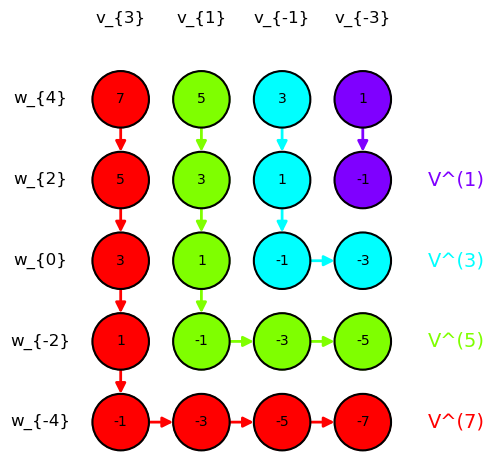
\includegraphics[width=0.6\textwidth]{figs/V4tensorV3graph.png}
\end{center}
Here we only draw the arrows representing the action of \(F\) (since \(E\) arrows point in the opposite direction, and the \(H\) eigenvalues can be read directly). Each distinct path corresponds to one irreducible component, verifying the Clebsch-Gordan decomposition:
\[
V^{(4)}\ox V^{(3)} \cong V^{(7)} \oplus V^{(5)} \oplus V^{(3)} \oplus V^{(1)}.
\]
\end{Ex}

\begin{Ej}
    Try your hand at computing \((V^{(1)})^{\otimes 3}\).
\end{Ej}

\section{Connection with \(\set{1,2}\)-words}

A word in the alphabet \(\set{1,2}\) is a string comprised of only those two characters. 

\begin{Ex}
The strings \(12221112121\), \(22221112121\), and \(22212112211\) are valid words!
\end{Ex}

We may connect these words to the standard representation \(V^{(1)}\) of \(\gsl_2\) via the correspondence for the basis vectors \(
1\leftrightarrow v_1,\quad 2\leftrightarrow v_{-1}\).\par
Thus, a word of length \(n\) corresponds directly to a basis vector in the \(n\)-fold tensor product \((V^{(1)})^{\otimes n}\).

The lowering operator \(F\) acts on these words as follows:
\begin{enumerate}
    \item Replace all \(1\)'s with right parentheses \()\) and all \(2\)'s with left parentheses \((\).
    \item Greedily match any adjacent parentheses pairs \(()\).
    \item The \(F\) operator finds the \textbf{rightmost unmatched \(1\)} (which corresponds to an unmatched \()\)) and turns it into a \(2\) (which is an \((\)). If there is no unmatched \(1\), \(F\) annihilates the word.
\end{enumerate}

The raising operator \(E\) acts in the opposite way.

\begin{Ej}
    Apply the \(F\) operator to the words \(211\), \(1122\), and \(12221112121\).
\end{Ej}

The complete connection with words is established by the following theorem:

\begin{Th}
    The irreducible representation \(V^{(n)}\) is isomorphic to the \(n^{\text{th}}\) symmetric power of the standard representation, \(\Sym^n(V^{(1)})\). 
\end{Th}

For example, this provides a clear correspondence between the weight diagram for \(V^{(3)}\) and the crystal graph for words of length 3:

\begin{center}
    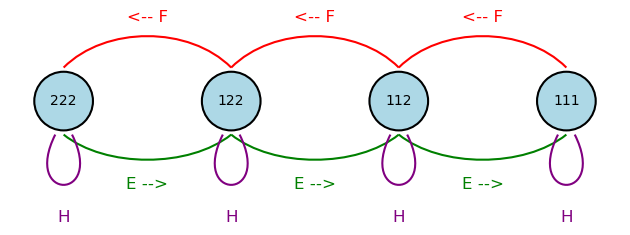
\includegraphics[width=0.6\textwidth]{figs/V3graphWords.png}
\end{center}

\begin{Ej}
    Try your hand at drawing the word graphs corresponding to the decomposition into irreducibles of \((V^{(1)})^{\otimes 3}\).
\end{Ej}


\end{document}
